
\chapter{User Walkthroughs}\label{app:user-walkthrough}

This section will go through each of the acceptance tests outlined in Section~\ref{sec:acc-tests} and provide the evidence that they pass. This evidence will be given in the form of:

\begin{itemize}
  \item Smart contract transaction logs from the Sepolia test-net. These are public at \small\url{https://sepolia.etherscan.io/address/0x2899dab55a4a20d698062bbf4d4ce9f1073ce052}\normalsize.
  \item Copies of particular log entries that correspond to specific actions.
  \item Screenshots to show changes being reflected in the user interface.
\end{itemize}

\newparagraph
For this the game will be a simple folder of text files that we can easily compare to show correctness. Any comparisons will be done using the \textit{diff} command. The games used will be:

\small
\begin{itemize}
  \item \g{1} = [title="User WT", version="1.0", developer="tcs1g20",\newline uploader=0xfBC8D99Bb9ab8F781fF04F9b45Fe5c97AACE1916, previousVersion=None, price=0, rootHash=`']
  \item \g{2} = [title="User WT", version="2.0", developer="tcs1g20", previousVersion=\g{1}, price=0,\newline uploader=0xfBC8D99Bb9ab8F781fF04F9b45Fe5c97AACE1916, rootHash=`']
\end{itemize}
\normalsize


\chapter{Introduction}\label{sec:problem}

Millions of worldwide users enjoy video games, which are large pieces of software that require complex platforms to distribute them, which results in them being generally provided by multinational corporations. However this approach often results in these platforms:

\begin{itemize}
  \item taking a large cut of revenue from developers\footnote{Steam take a 30\% cut~\cite{marks_report_2019,brown_valve_2021}},
  \item being prone to censorship from entities like governments\footnote{See the Chinese version of Steam~\cite{noauthor_steam_nodate-1}},
  \item relying on a single platform to stay active, distribute games and maintain a user's ownership\footnote{The Nintendo eShop closing down prevents users from accessing games~\cite{noauthor_nintendo_2022}}.
\end{itemize}

\section{Objectives}

Modern web ideas revolve around taking power away from large corporations and having platforms that are built, run and maintained by those who use them.
This project aims to produce a proof-of-concept, distributed video game marketplace that will allow developers to continuously release and update their games on a public network such that they can be purchased and downloaded by other users.

\section{Scope}

This project will strictly focus on creating a distributed platform in which users can upload, purchase and share games and will consist of the following components:

\begin{enumerate}
  \item An Ethereum smart contract that will allow us to maintain a library of games that can be queried and added to by any user. This will then be deployed to an Ethereum test-net.
  \item A local application to be run by users to interact with the smart contract and allow them to join a peer-to-peer network where they can download and upload games.
\end{enumerate}

\newparagraph
This project will not present methods for preventing or stopping the distribution of illegal content or include tangentially related features such as achievements, or message boards.

\chapter{Background Research}

This chapter describes two distributed-web technologies that allows user to connect over large, decentralised networks and overcome issues of distributing data and building trust.


\section{BitTorrent}

BitTorrent~\cite{kaune_unraveling_2010,pouwelse_bittorrent_2005} is the most popular p2p file-sharing platform, in which users will barter for chunks of files by downloading and uploading them in a tit-for-tat fashion, such that peers with a high upload rate will typically also have a high download rate. For a user to download data from BitTorrent they would:

\subsection{Download Protocol}

\begin{enumerate}
  \item Find the corresponding \.torrent file that contains metadata about the torrent such as the location of a tracker, file information such as name, size and path in the directory.
  \item The user will find peers also interested in that torrent through a tracker and will establish connections with them.
  \item The data is split into constant-sized blocks and are downloaded individually. BitTorrent uses a tit-for-tat mechanism that incentivises users to contribute by providing preferable treatment to nodes who upload data as well.
  \item The user will download blocks based upon the following priority:
        \begin{enumerate}
          \item \textbf{Strict Priority} Data is split into pieces and sub-pieces with the aim that once a given sub-piece is requested then all of the other sub-pieces in the same piece are requested
          \item \textbf{Rarest First} Aims to download the piece that the fewest peers have to increase supply.
          \item \textbf{Random First Piece} When a peer has no pieces, it will try to get one as soon as possible to be able to contribute.
        \end{enumerate}
  \item The node will continuously upload blocks it has while active.
\end{enumerate}

\subsection{Availability}

It is commonly suggested that availability of torrents is the biggest issue surrounding BitTorrent as \textit{`38\% of torrents become unavailable in the first month'}~\cite{kaune_unraveling_2010} and that \textit{`the majority of users disconnect from the network within a few hours after the download has finished'}~\cite{pouwelse_bittorrent_2005}.
This paper~\cite{neglia_availability_2007} looks at how the use of multiple trackers for the same content and DHTs can be used to boost availability.



\section{Ethereum}

Ethereum is a Turing-complete, distributed, transaction-based blockchain that allows the deployment of decentralized applications through the use of smart contracts. Ether is the currency used on Ethereum and can be traded between accounts and is used to execute smart contract code on the network. 

\subsection*{Smart Contracts}

A smart contract is an executable piece of code, written in Solidity, that will automatically execute on every node in the Ethereum network when certain conditions are met. Smart contracts are enforced by the blockchain network and remove the need for intermediaries and reduce the potential of contractual disputes.
\x
Gas is used to measure the computational effort of running a smart contract and must be paid, in Ether, before being processed and added to the blockchain. This helps prevent DoS attacks and provides economic incentives for users to behave in a way that benefits the whole network.

\subsection*{Example Use Cases}

Some examples of applications that can be deployed to the Ethereum network are:

\begin{itemize}
  \item Financial applications, such as decentralised exchanges and payment systems,
  \item supply chain management and tracking,
  \item voting and governance systems,
  \item unique digital asset systems, and
  \item data storage and sharing platforms.
\end{itemize}

\chapter{Project Management}

\subsection*{Risk Assessment}

% \paragraph*{Difficult with blockchain development}

% Some of the difficulties I found with blockchain development were:

% \begin{itemize}
%   \item 
% \end{itemize}

\paragraph*{The application is not finished}
Section~\ref{tab:sprint-3} shows the scoped requirements that were not met and Section~\ref{sec:design-lim} shows some of the limitations within my design when compared to similar platforms. However, use of MoSCoW prioritisation and sprint planning meant I was still able to produce a largely functional application that met the majority of the requirements and having a cut off point for implementation ensured I had sufficient time to complete this report.
\x
One reason for not finishing was the size of the project, which took a considerable amount of time to implement and test. Table~\ref{tab:cloc} shows a breakdown of the source code.

\begin{longtable}{ r r r r }
  \toprule
  \textbf{Language} & \textbf{Files} & \textbf{Comments} & \textbf{Code}
  \\\midrule\midrule
  Go
  & 44
  & 683
  & 4621
  \\
  Go Tests
  & 29
  & 791
  & 3205
  \\
  Vue.js Components
  & 18
  & 147
  & 2855
  \\
  JavaScript
  & 19
  & 74
  & 209
  \\
  Solidity
  & 1
  & 30
  & 51
  \\\bottomrule\bottomrule
  \caption{The lines of code written for this project calculated using CLOC~\cite{noauthor_aldanialcloc_nodate} excluding any auto-generated code.}
  \label{tab:cloc}
\end{longtable}

\paragraph*{Lack of large-scale testing infrastructure}
Testing distributed applications is challenging due to many factors, such as having to source homogenous devices, having access to networks that would allow me host a peer, and more. However, several useful results were produced from the benchmarks (Section~\ref{sec:benchmark}) and acceptance tests (Section~\ref{sec:acc-tests}) that can be used to improve the application. If this project were to move forward then testing it on a large-scale would be essential.
\section{Sprint Plans}

\newcommand{\yes}{\cellcolor{green!30}YES}
\newcommand{\started}{\cellcolor{yellow!50}STARTED}
\newcommand{\no}{\cellcolor{red!30}NO}

The use of sprints was essential in managing my time and ensuring that I was working on the most important aspects of my project first. The use of MoSCoW priortisation and by then dividing my requirements into logical groups I was able to effectively target key aspects of my application in bulk. The use of test-driven development~\cite{beck_test-driven_2003} meant that at the end of each sprint, each piece of code I wrote was tested and I could move on.
\x
For each sprint we will detail the planned requirements, whether they were completed or not, as well as any general comments about that sprint.

\subsection{Sprint 1}

I anticipated that the P2P game distribution network would be the most complex and time consuming set of requirements in this project so I decided to focus on it for this first sprint. Table~\ref{tab:sprint-1} shows the requirements included for Sprint 1 and whether they were completed or not.
\x
This sprint was largely problem-free as I didn't have much to learn to be able to complete this and could rely heavily on my design to structure my implementation.

\begin{longtable}{p{0.12\textwidth} p{.13\textwidth} p{.6\textwidth}}
  \toprule
  \textbf{Req.} & \textbf{Complete} & \textbf{Evidence/Reasoning}
  \\\midrule\midrule
  \reqref{F-M7}
  & \yes
  & Unit tests for the model/net/tcp package and the peer count benchmark tests.
  \\
  \reqref{F-M8}
  & \yes
  & Unit tests for the model/net/peer/message\_handlers file test the handling of structured messages and the structured responses sent back. 
  \\
  \reqref{F-M9}
  & \yes
  & All benchmark tests show the downloading of data to a large scale.
  \\
  \reqref{F-M10}
  & \yes
  & Unit tests to show incorrect messages being rejected.
  \\
  \reqref{F-M11}
  & \yes
  & User walkthrough shows the download of a game in its entirety. 
  \\
  \reqref{F-M12}
  & \started
  & The algorithm to generate a hash tree and the using of it to download data was implemented but no way to upload it anywhere.
  \\\midrule\midrule
  \reqref{NF-M2}
  & \yes
  & User walkthrough ... shows that any user can establish a connection with any other user.
  \\
  \reqref{NF-S1}
  & \started
  & Users will form many connections concurrently and optimisations were made using the producer/consumer pattern to complete actions like inserting data, or reqeusting data.
  \\\bottomrule\bottomrule
  \caption{Requirements included for Sprint 1}
  \label{tab:sprint-1}
\end{longtable}

\subsection{Sprint 2}

Sprint 2 was about increasing the scope of the application by focusing on two main aspects:

\begin{enumerate}
  \item The integration with Ethereum using a Smart Contract, and
  \item Allowing users to interface with the application via a GUI.
\end{enumerate}

\vspace{2mm}\noindent
This sprint had a much slower start compared to the first one as I was largely unfamiliar with smart contract development and the related packages needed to interface with them. On top of this, I considered several UI framework's before settling on my final choice which increased the length of this sprint.
\x
Table~\ref{tab:sprint-2} shows the requirements pitched for Sprint 2 and whether or not they were completed.

\begin{longtable}{p{0.12\textwidth} p{.13\textwidth} p{.6\textwidth}}
  \toprule
  \textbf{Req.} & \textbf{Complete} & \textbf{Evidence/Reasoning}
  \\\midrule\midrule
  \reqref{F-M1}
  & \yes
  & Unit tests for the Library smart contract and user walkthrough ... show the ability to upload game metadata to Ethereum.
  \\
  \reqref{F-M2}
  & \yes
  & Unit tests for the Library smart contract and user walkthrough ... show the ability to upload an update to an existing game to Ethereum.
  \\
  \reqref{F-M3}
  & \yes
  & Unit tests for the Library smart contract show users of an existing game being given ownership of an updated version.
  \\
  \reqref{F-M4}
  & \yes
  & The smart contract was successfully deployed the Sepolia test-net~\cite{etherscanio_deployed_nodate}. All user walkthroughs will form connections to this smart contract.\\
  \reqref{F-M5}
  & \yes
  & Unit tests for the Library smart contract and user walkthrough ... show the successful purchase of a game.
  \\
  \reqref{F-M6}
  & \yes
  & Unit tests for the Library smart contract show a user being added to a mapping containing all users who have purchased the game.
  \\
  \reqref{F-M12}
  & \yes
  & Hash trees are now uploaded to IPFS and the CID is stored on Ethereum. 
  \\
  \reqref{F-S2}
  & \started
  & Basic pages were added according to Section~\ref{subsubsec:frontend}. These pages had little styling or reactivity but could perform the required basic functions. See Appendix~\ref{app:screenshots} for screenshots of the final versions.
  \\\midrule\midrule
  \reqref{NF-M1}
  & \yes
  & The use of the Ethereum blockchain means that no single user can control what is uploaded to the network.
  \\
  \reqref{NF-M3}
  & \yes
  & Developers can be uniquely identified using their Ethereum address. This should be made publically verifiable by the developers.
  \\
  \reqref{NF-M4}
  & \yes
  & Data stored on Ethereum is inherently immutable.
  \\
  \reqref{NF-M5}
  & \yes
  & Unit tests for the smart contract show the restriction that only the original uploader can release an update.
  \\\bottomrule\bottomrule
  \caption{Requirements included for Sprint 2}
  \label{tab:sprint-2}
\end{longtable}

\subsection{Sprint 3}

\begin{longtable}{p{0.12\textwidth} p{.13\textwidth} p{.6\textwidth}}
  \toprule
  \textbf{Req.} & \textbf{Complete} & \textbf{Evidence/Reasoning}
  \\\midrule\midrule
  \reqref{F-S1}
  & \yes
  & Users will validate each other's Ethereum address after forming a connection and unit tests for the model/net/peer/message\_handlers file show this being performed.
  \\
  \reqref{F-S2}
  & \yes
  & The UI was overall improved to improve the user experience.
  \\
  \reqref{F-S3}
  & \no
  & Users will track the blocks sent to them by each of their peers but this application has no mechanism for redeeming these. Due to time constraints, I was unable to implement a sufficient solution. Moreover, I felt that a micro-payment system, like present in Swam~\cite{hartman_swarm_1999}, would be a much better implementation.
  \\
  \reqref{F-S4}
  & \yes
  & Users will exchange the REQ\_PEERS/PEER commands to discover neighbouring peers.\newline
  However a better implementation might have the developer of the game be able to provide a list of peers who have the game. This would allow a user to easily find peers who are interested in the same content.
  \\
  \reqref{F-C1}
  & \no
  & Due to time constraints I was unable to implement this at all.
  \\
  \reqref{F-C2}
  & \yes
  & Game assets are uploaded to IPFS and the CID is stored with the game metadata on Ethereum.
  \\\midrule\midrule
  \reqref{NF-S1}
  & \yes
  & Benchmark tests show the scalability of my application by varying certain parameters and that the target file size can be downloaded within an acceptable best-case.
  \\
  \reqref{NF-S2}
  & \yes
  & Changes to the UI made it more interactive and easier to navigate. Designs were inspired by pages from existing platforms to make the UI feel familiar. See Appendix~\ref{app:screenshots} for screenshots of the final versions.
  \\
  \reqref{NF-C1}
  & \no
  & Completing this requirement would be incredibly complex and was decided against being completed. Preventing the distribution of illegal content is an important consideration moving forward to help keep the platform safe.
  \\
  \reqref{NF-C2}
  & \yes
  & A help page was included answering some questions that new users may have about the application.
  \\\bottomrule\bottomrule
  \caption{Requirements included for Sprint 3}
  \label{tab:sprint-3}
\end{longtable}


\section{Gantt Chart}

A Gantt chart was used to give myself a high-level overview of how my time should be spent so that I would have appropriate time to complete the necessary aspects of this project. This was useful in prioritising different aspects and knowing when to plan deadlines for myself (for example, having a hard cut-off point for my implementation).
\x
Figure~\ref{fig:gantt-chart-1} shows the Gantt chart for this project up util the progress report submission, which includes the planning and design phases.

\begin{figure}[H]
  \centering
  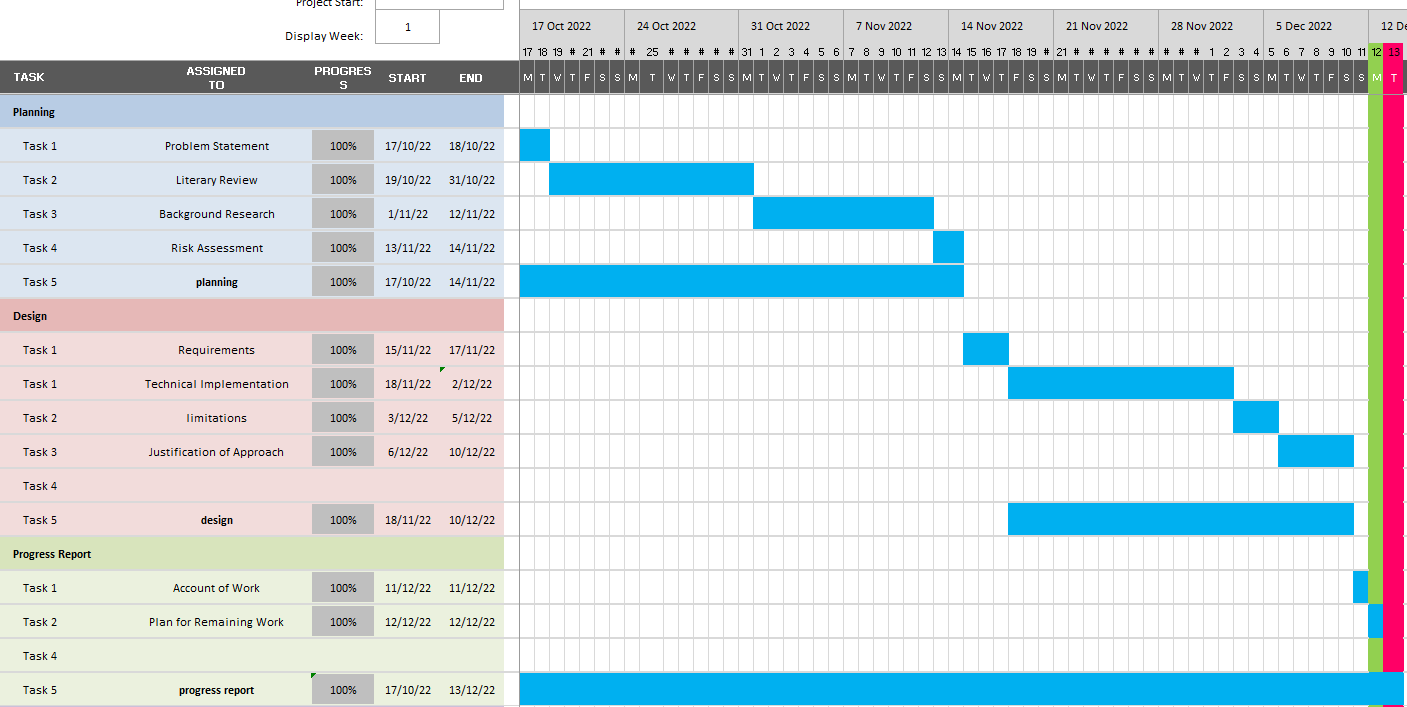
\includegraphics[width=\textwidth]{assets/images/charts/gantt/progress.png}
  \caption{Gantt Chart leading up to the progress report}
  \label{fig:gantt-chart-1}
\end{figure}

\noindent Figure~\ref{fig:gantt-chart-2} shows the Gantt chart for the implementation phase of this project. The implementation phase was split into three sprints, as detailed in Section~\ref{sec:sprints}, each with their own planning phase.

\begin{figure}[H]
  \centering
  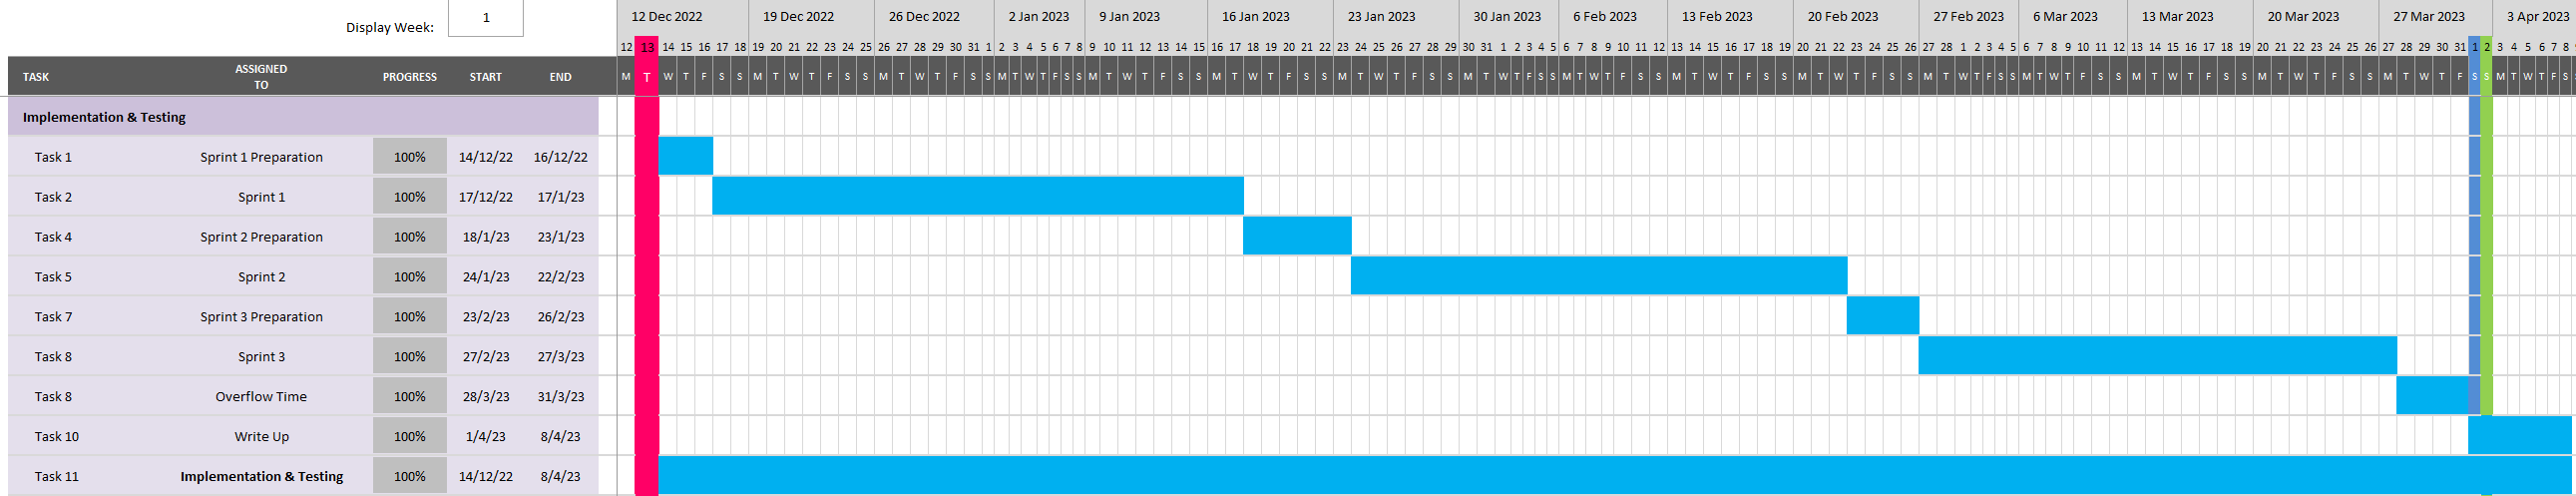
\includegraphics[width=\textwidth]{assets/images/charts/gantt/impl.png}
  \caption{Gantt Chart showing the three sprints}
  \label{fig:gantt-chart-2}
\end{figure}

\noindent Figure~\ref{fig:gantt-chart-3} shows the Gantt chart for the final testing and evaluation phases of my application. As I used test-driven development, the testing phase only needed to consist of acceptance and benchmark testing among some other fixes. 

\begin{figure}[H]
  \centering
  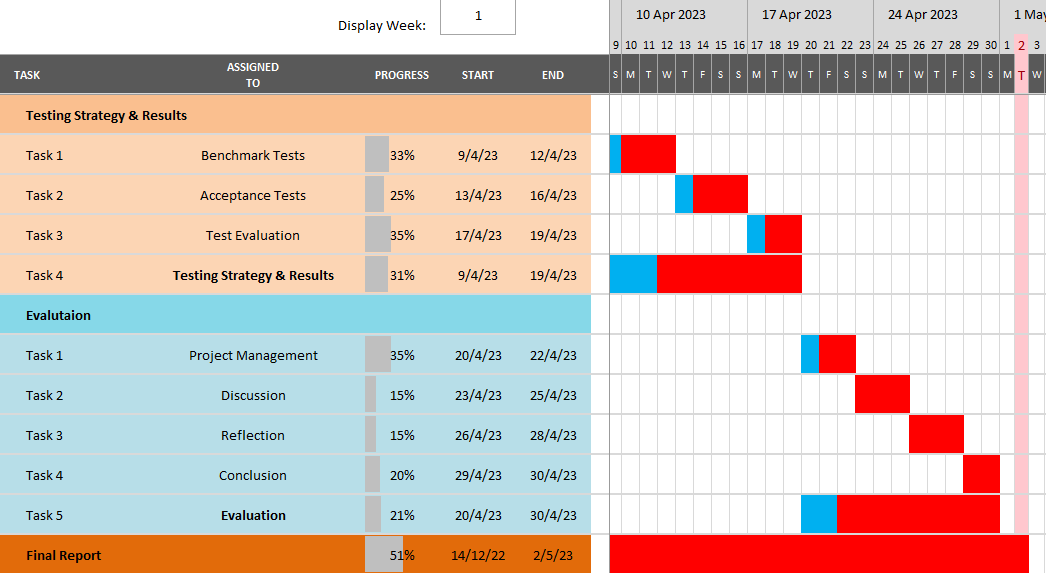
\includegraphics[width=\textwidth]{assets/images/charts/gantt/testing-eval.png}
  \caption{Gantt Chart showing the final testing and evaluation}
  \label{fig:gantt-chart-3}
\end{figure}
% \section{Work to Date}

My work has primarily been on research, looking at how blockchain has been used to build and supplement cloud storage systems as well as how various peer-to-peer functioned and performed. 
I have proposed a design for the application to be built on the EVM. 

\begin{figure}[ht]
  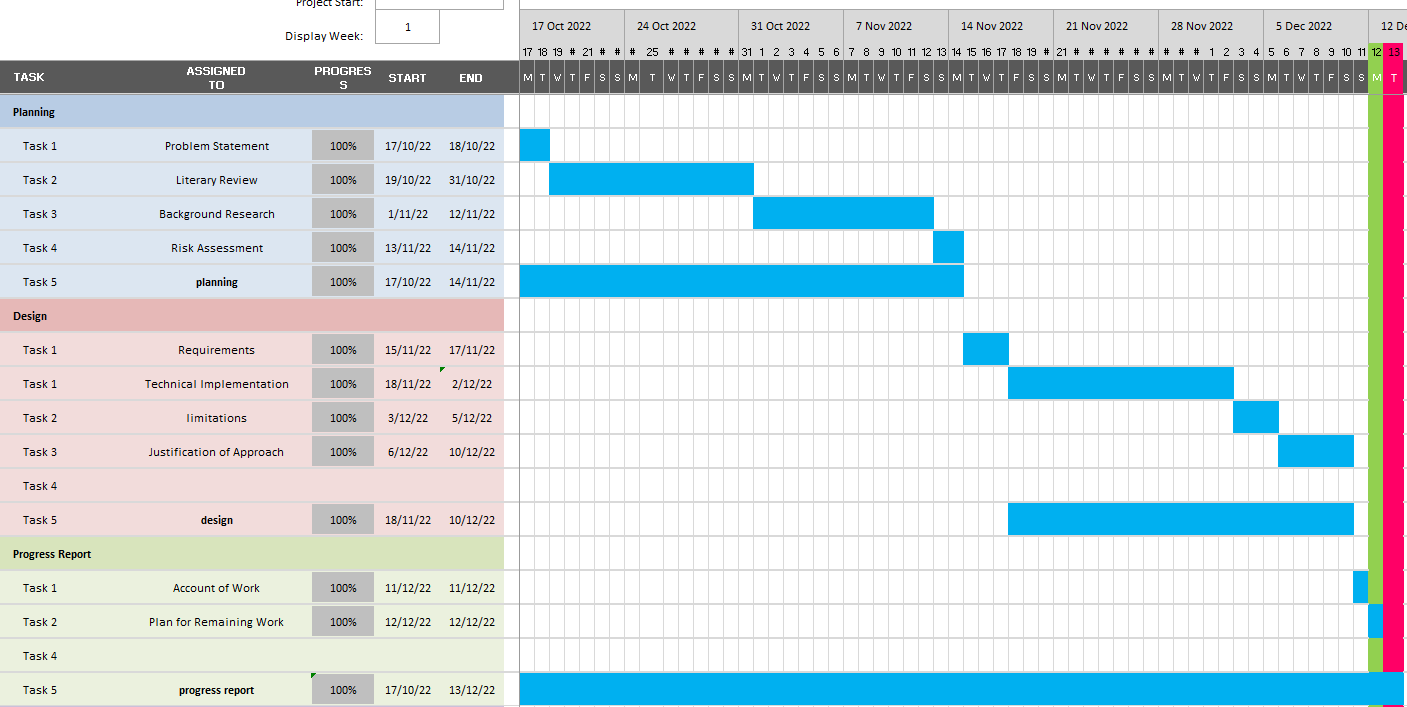
\includegraphics[width=\textwidth]{assets/images/charts/gantt/progress.png}
  \caption{A Gantt chart for my work up until the progress report.}
\end{figure}

% \section{Plan of Future Work}

Below is a high level plan of the work I have remaining. At the end of each section, I will write up the initial draft of that section in my final report based upon notes made throughout the project.

\subsection*{Implementation \& Testing}
This phase I will use the agile development methodology to build my application. My sprints will all be structured into three phases:
\vspace{1mm}

\begin{enumerate}
  \item \textbf{Preparation} Deciding on the set of requirements to complete and making any initial design decisions and diagrams,
  \item \textbf{Implementation} using test-driven development, I will work on requirements based on their prioritization, and
  \item \textbf{Review} I will discuss the completed work in that sprint including design choices, what was completed, and any issues.  
\end{enumerate}

\vspace{1mm}\noindent By using a preparation and review phase with each sprint, I can make detailed notes on my implementation as I go so when I come to write the full report I have a strong starting point.

\begin{figure}[ht]
  \centering
  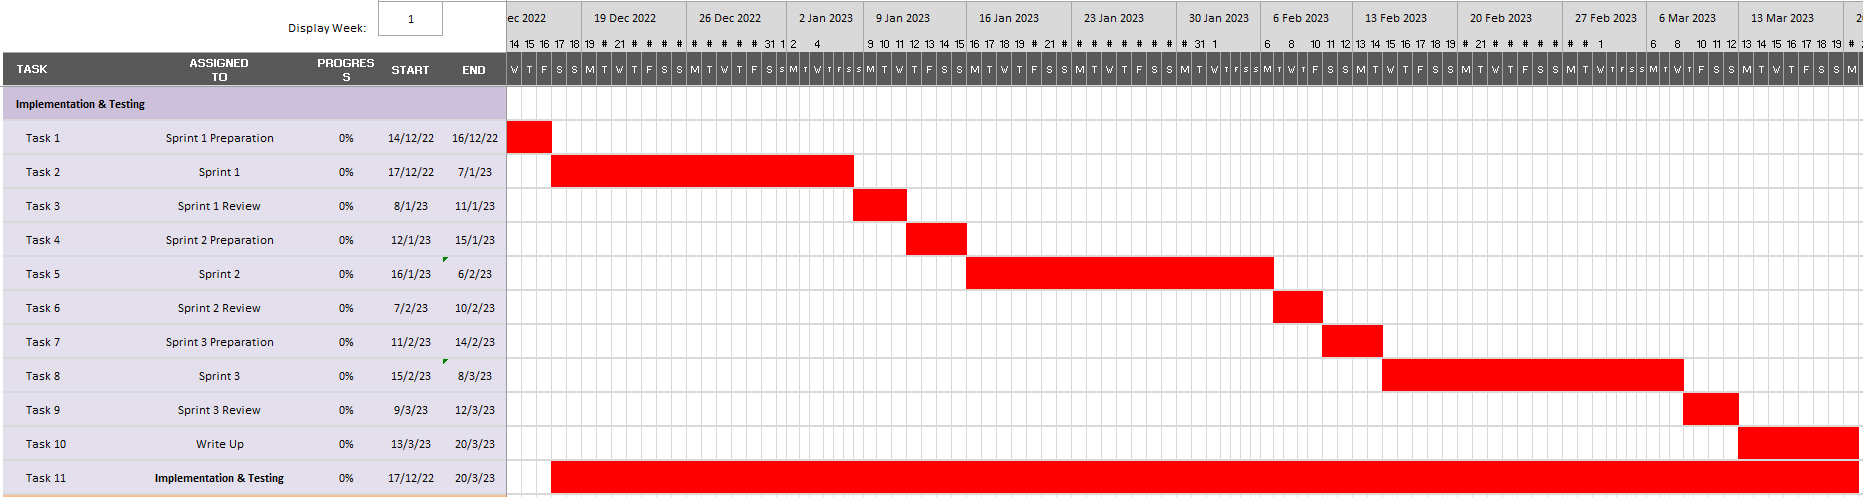
\includegraphics[width=\textwidth]{assets/images/charts/gantt/implementation-testing.png}
  \caption{The plan for my three sprints}
\end{figure}

\subsection*{Testing Strategy and Results}
This phase will consists of several sections:

\begin{enumerate}
  \item \textbf{Testing Strategy} The approach I used for writing tests throughout the implementation phase and how these were used to evaluate the completion of the requirements set out in Section~\ref{subsec:requirements}. 
  \item \textbf{Test Results} A report on the results of my automated and manual testing.
\end{enumerate}

\subsection*{Evaluation}
This phase will have me evaluating how successful my project was, as a whole, by focusing on several key areas:

\begin{enumerate}
  \item \textbf{Project Organisation} How successfully did I structure my time in this project?
  \item \textbf{Outcome of the Application} How successful was my application in regards to a solution to the problem set out in Section~\ref{sec:problem} and in terms of the requirements set out in Section~\ref{subsec:requirements}?
  \item \textbf{Limitations and Future Improvements} What were the limitations of my project and what would I change about it if I had more time or were to start again?
\end{enumerate}

\begin{figure}[ht]
  \centering
  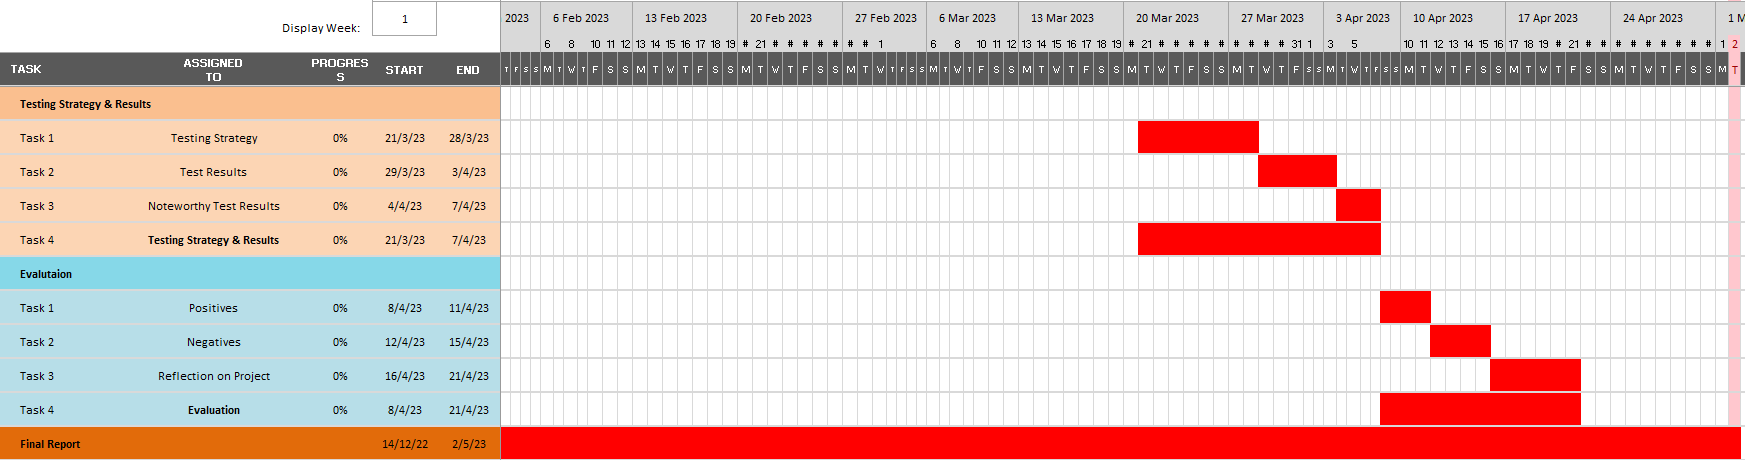
\includegraphics[width=\textwidth]{assets/images/charts/gantt/testing-evaluation.png}
  \caption{The plan for my testing and evaluation phases}
  \label{fig:final-gantt}
\end{figure}

\subsection*{Leftover Time}

At the end of my project, I've left some time unallocated to account for certain tasks that may take longer as well as the writing up of my final report. This should leave me with an acceptable amount of time to finish the project despite some setbacks.


\chapter{Literature Review}\label{ch:lit-review}

This section will be used to examine the literature surrounding the distributed storage of data. Initially I will look at various distributed file-sharing protocols and then how blockchain has been used to enhance them.


\section{P2P File Sharing}

These applications involve a distributed network of computers that share data with each other without the need for a central party. Table~\ref{tab:lit-review-p2p} shows some example p2p file-sharing networks.
\x
One of the main issues with these networks come from their anonymity property in that you can never fully trust that what you're downloading isn't malicious. On top of this, these platforms don't offer a way for user to pay for the content they are downloading, which means that legal, proprietary content is rarely distributed over them.

\begin{longtable}{ p{0.15\textwidth} p{0.8\textwidth} }
  \toprule
  \textbf{System} & \textbf{Description of Solution}
  \\\midrule\midrule
  IPFS~\cite{benet_ipfs_2014}
  & IPFS is a content-addressable, block storage system which forms a Merkle DAG, a data structure that allows the construction of versioned file systems, blockchains and a Permanent Web.
  %
  \x
  BitTorrent~\cite{pouwelse_bittorrent_2005}
  & BitTorrent is a p2p file-sharing system that has user bartering for chunks of data in a tit-for-tat fashion, which provides incentive for users to contribute to the network. More on BitTorrent can be found in Section~\ref{sec:bittorrent}
  %
  \x
  AFS~\cite{morris_andrew_1986,howard_scale_1988}
  & The Andrew File System was a prototype distributed system by IBM and Carnegie-Mellon University in the 1980s that allowed users to access their files from any computer in the network.
  %
  \x
  Napster~\cite{saroiu_measurement_2001}
  & Napster uses a cluster of centralized servers to maintain an index of every file currently available and which peers have access to it. A node will maintain a connection to this central server and will query it to find files; the server responds with a list of peers and their bandwidth and the node will form a connection with one or many of them and download the data.
  %
  \x
  Gnutella~\cite{saroiu_measurement_2001}
  & Gnutella nodes form an overlay network by sending \textit{ping-pong} messages. When a node sends a \textit{ping} message to their peers, each of them replies with a \textit{pong} message and the \textit{ping} is forwarded to their peers. To download a file, a node will flood a message to its neighbors, who will check if they have and return a message saying so; regardless, the node will continue to flood their request till they find a suitable node to download off of.
  \\\bottomrule
  \caption{\textit{Various global distributed file systems.}}
  \label{tab:lit-review-p2p}
\end{longtable}

\section{Blockchain-Based Cloud Storage}

In table~\ref{tab:blockhain cloud storage}, I detail some examples of how blockchain has been used to solve problems within cloud storage systems. One interesting finding from these papers~\cite{sukhodolskiy_blockchain-based_2018,hasan_cloud_2019} is that blockchain can been used to provide additional services to cloud storage systems, such as monitoring access control or helping to verify the integrity of the data on these systems.

\begin{longtable}{ p{0.35\textwidth} p{0.6\textwidth} }
  \toprule
  \textbf{Paper} & \textbf{Description of Solution}
  \\\midrule\midrule
  Blockchain Based Data Integrity Verification in P2P Cloud Storage~\cite{yue_blockchain_2018}
  & This paper uses Merkle trees to help verify the integrity of data within a P2P blockchain cloud storage network as well as looking at how different structures of Merkle trees effect the performance of the system.
  %
  \x
  Deduplication with Blockchain for Secure Cloud Storage~\cite{li_deduplication_2018}
  & This paper describes a deduplication scheme that uses the blockchain to record storage information and distribute files to multiple servers. This is implemented as a set of smart contracts.
  %
  \x
  Block-secure: Blockchain based scheme for secure P2P cloud storage~\cite{li_block-secure_2018}
  & A distributed cloud system in which users divide their own data into encrypted chunks and upload those chunks randomly into the blockchain, P2P network. 
  %
  \x
  Blockchain-Based Medical Records Secure Storage and Medical Service Framework~\cite{chen_blockchain-based_2018}
  & Describes a secure and immutable storage scheme to manage personal medical records as well as a service framework to allow for the sharing of these records.
  %
  \x
  A Blockchain-Based Access Control System for Cloud Storage~\cite{sukhodolskiy_blockchain-based_2018}
  & This paper describes a method for using blockchain to facilitate the access control over a cloud storage system. The blockchain stores an immutable record of all `\textit{meaningful security events}', such as key generation, access policy, assignment, etc.
  %
  \x
  Cloud Data Provenance using IPFS and Blockchain Technology~\cite{hasan_cloud_2019}
  & Uses blockchain technology and IPFS to provide an efficient way to securely store provenance~\footnote{Provenance data are access logs of stored data that can trace the integrity of data and will contain private user information.} data such that it is out of reach of adversaries, but can be used to verify the integrity of data on a cloud storage system. 
  \\\bottomrule\bottomrule
  \caption{\textit{Examples of blockchain cloud storage systems~\cite{sharma_blockchain_2021} }}
  \label{tab:blockhain cloud storage}
\end{longtable}



\section{Overview}
\chapter{Design}



\subsection{Stakeholders}

\newcommand{\primary}{\hlc{cyan}{ PRIMARY }\\}
\newcommand{\secondary}{\hlc{yellow}{ SECONDARY }\\}
\newcommand{\tertiary}{\hlc{green}{ TERTIARY }\\}

\paragraph{Game Developers}\primary
This group will use the application to release their games and its updates to their users, who they will reward for helping to distribute it.

\paragraph{Players}\primary
This group will use this application to downloaded and update their games off of. They may also contribute to the distribution of the games to other players for an incentive provided by the developers.

\paragraph{Game Distribution Platforms}\secondary
This group consists of platforms like Steam or Epic Games, which serve as the main competitor to this application. It is likely that as more developers choose this application, this group will see a loss in revenue. 

\paragraph{}\tertiary

\section{Stakeholders \& Requirements}

\input{sections/5-design/stakeholders.tex}

\subsection{Requirements}

Tables~\ref{tab:functional-requirements} and~\ref{tab:non-functional-requirements} show the functional and non-functional requirements of this project organized using MoSCoW prioritisation. 

\subsubsection*{Functional Requirements}

\begin{longtable}{ p{.1\textwidth} p{.8\textwidth} }
  \toprule
  \textbf{ID} & \textbf{Description}
  \\\midrule\midrule
  \multicolumn{2}{c}{\cellcolor{red!70}\textit{Must}}\\\midrule
  F\_M1 & Store software metadata on a blockchain\\
  F\_M2 & A node must request individual shards from its peers\\
  F\_M3 & A node must be able to discover peers relevant to the software it wants\\
  F\_M4 & Software must be updatable through the blockchain\\
  F\_M5 & A node must be able to upload software\\
  F\_M6 & A node must be able to download software in its entirety from nodes in the same network.\\
  F\_M7 & A node must be able to verify the integrity of each block it downloads\\
  F\_M8 & The application should run on the Ethereum network\\
  F\_M9 & Users must be able to purchase games from developers over the network\\
  F\_M10 & Users must be able to prove they have purchased a game\\
  \midrule\multicolumn{2}{c}{\cellcolor{orange!70}\textit{Should}}\\\midrule
  F\_S1 & Seeders should have a way to prove how much data they have seeded\\
  F\_S2 & Seeders will only upload content to users who have a valid proof of purchase\\
  \midrule\multicolumn{2}{c}{\cellcolor{green}\textit{Could}}\\\midrule
  F\_C1 & Allow users to request specific software versions\\
  \midrule
  \bottomrule
  \label{tab:functional-requirements}
\end{longtable}

\subsubsection*{Non-Functional Requirements}

\begin{longtable}{ p{.1\textwidth} p{.8\textwidth} }
  \toprule
  \textbf{ID} & \textbf{Description}
  \\\midrule\midrule
  \multicolumn{2}{c}{\cellcolor{red!70}\textit{Must}}\\\midrule
  NF\_M1 & The application is decentralized and cannot be controlled by any one party\\
  NF\_M2 & Any user must be able to join and contribute to the network\\
  NF\_M3 & Game uploaders should be publicly identifiable\\
  NF\_M4 & Metadata required to download the game should be immutable\\
  \midrule\multicolumn{2}{c}{\cellcolor{orange!70}\textit{Should}}\\\midrule
  NF\_S1 & This application must be scalable, such that many users can upload and download the same game at the same time.\\
  NF\_S2 & Only the original uploader can upload an update to their game\\
  \midrule\multicolumn{2}{c}{\cellcolor{green}\textit{Could}}\\\midrule
  \\
  \midrule
  \bottomrule
  \label{tab:non-functional-requirements}
\end{longtable}

\section{Design Considerations}

This section will give a high-level design showing how each of the functional requirements can be met by considering key functions for the applications.

% chktex-file 24
% chktex-file 8

\subsection{Data}
\label{subsec:design-data}

Table~\ref{tab:data} discusses the different types of data we are going to need to store and where they should be stored based upon their properties.


\begin{longtable}{ p{.12\textwidth} p{.1\textwidth} p{.1\textwidth} p{.63\textwidth} }
  \toprule
  \textbf{Data} & \textbf{Size} & \textbf{Location} & \textbf{Explanation}\\
  \midrule\midrule
  Game Metadata\newline\reqref{F-M1}
  & 100 -- \newline200B
  & Ethereum
  & This data is the minimal set of information required for the unique identification of each game. See Section~\ref{subsubsec:eth-data}.

  \vspace{1mm}
  This data is appropriate to store on Ethereum as it is public, small in size, and essential to the correct functioning of the application as all users will need to be able to discover all games. 
  \x
  Game Hash Tree\newline\reqref{F-M12}
  & \~15KB
  & IPFS
  & This will be the compressed Hash Tree that will allow the users to identify and verify the shards of data they need to download for their game. The user will download this immediately after purchasing the game.

  \vspace{1mm}
  This data would be costly to store on Ethereum for a large number of games and will only need to be accessed by a subset of users. As it is also public data, IPFS is appropriate to store it on, and we can reference the CID within the data stored on Ethereum.
  \x
  Game\newline Assets\newline\reqref{F-C2}
  & Unkown~\footnote{Some games may include many promotional materials, whilst some could include none. Therefore, it is hard to estimate the expected size.} 
  & IPFS
  & This will represent any promotional material provided for the game that can be viewed on the game's store page. This will typically include cover art and a markdown file for the description. The user will download this when they first view it in the store.

  \vspace{1mm}
  Similar to the Hash Tree, this will typically be too large to store on Ethereum so, given that it is public and non-essential data, IPFS will be used to store and distribute it. 
  \x
  Game Data
  & \textit{avg. 44GB~\footnote{Calculated based off of the top 30 games from SteamDB~\cite{noauthor_steam_nodate}.}}
  & Peers
  & This will the data required to play the game and will be fetched based upon the contents of the game's Hash Tree.

  \vspace{1mm}
  This data is way too large to store on Ethereum but also isn't public, which means using IPFS would not be appropriate~\footnote{IPFS and similar platforms provide no access control for the data stored there and any encryption based technique would be unviable.}. Therefore, this project will use a custom P2P network for sharing data, which is described in Section~\ref{subsec:design-p2p} 
  \\\bottomrule\bottomrule
  \caption{The different types of data required for each game.}
  \label{tab:data}
\end{longtable}

\noindent 
Swarm~\cite{hartman_swarm_1999} was considered as a decentralised storage and distribution platform over IPFS but was decided against as it would couple this project more tightly with Ethereum. On top of that, IPFS has much greater adoption and is much more mature in terms of working on a large scale.

\subsection*{Blockchain}\label{subsec:design-con-eth}

\subsubsection*{Type of Blockchain}

To satisfy \reqref{NF-M1} and \reqref{NF-M2}, we will need to use a public blockchain. This will benefit my project by:
\vspace{2mm}
\begin{itemize}
  \item being accessible to more users, which will boost both availability and scalability \reqref{NF-S1},
  \item reducing the risk of censorship \reqref{NF-M1}, and
  \item providing greater data integrity \reqref{NF-M4}
\end{itemize}

\newparagraph Ethereum is a public blockchain that allows developers to publish their own distributed applications to it. It comes with an extensive development toolchain so is an obvious choice for this project \reqref{F-M4}.

\subsubsection*{Uploading Games}
\label{subsubsec:eth-data}



To satisfy \reqref{F-M1} and \reqref{F-M2}, the data stored on the blockchain will be used for the identification of games. Table~\ref{tab:eth-data} shows the fields that will stored as part of the smart contract for each game and to manage the whole collection of games. Fields in \textit{italics} are generated for the user and non-italic fields are entered manually.

\begin{longtable}{ p{.2\textwidth} p{.75\textwidth} }
  \toprule
  \textbf{Name} & \textbf{Description}
  \\\midrule\midrule
  \multicolumn{2}{c}{\textit{Metadata for each game}} 
  \\\midrule\midrule
  title & The name of the game.\\
  version & The version number of the game.\\
  \textit{release date} & The timestamp for when the game was uploaded.\\
  developer & The name of the developer uploading the game \reqref{NF-M3}.\\
  \textit{uploader} & The Ethereum address of the developer \reqref{NF-M3}.\\
  \textit{root hash} & The root hash of the game that uniquely identifies the game and is based upon its contents.\\
  previous version & The root hash of the most previous version of the game if it exists.\\
  price & The price of the game in Wei.\\
  \textit{hash tree CID} & Required for downloading the hash tree from IPFS.\\
  \textit{assets CID} & Required for downloading the assets folder from IPFS.
  \\\midrule\midrule
  \multicolumn{2}{c}{\textit{Managing the Collection of Games}} 
  \\\midrule\midrule
  \textit{library} & A mapping for all games uploaded to the network, where a game's root hash is the key used to find its metadata.\\
  \textit{game hashes} & Solidity doesn't allow us to enumerate maps so we will also store a list of hashes for all games uploaded.\\
  \textit{purchased} & A mapping which allows us to easily check if a user has purchased a game \reqref{F-M6}.
  \\\bottomrule\bottomrule
  \caption{the data to be stored on Ethereum using a smart contract}
  \label{tab:eth-data}
\end{longtable}


\subsubsection*{Purchasing Content}

Users will purchase games from developers over Ethereum by transferring Ether \reqref{F-M5}. The user's address will then be added to a public record, on the smart contract, of all users who have purchased the game \reqref{F-M6}. Upon purchasing a game, a user will broadcast their new library to all of their peers.

% chktex-file 1
% chktex-file 13

\subsection{Distributed File Sharing}
\label{subsec:design-p2p}

\subsubsection*{Hash Tree}
\label{subsubsec:hash-tree}

The hash tree of a given directory is used to represent its structure as well as the contents of its files. Each file is represented by an ordered list of SHA-256 hashes that match a fixed-size block of data. This allows users to easily identify and verify game data \reqref{F-M10}.

\begin{figure}[ht]
  \centering
  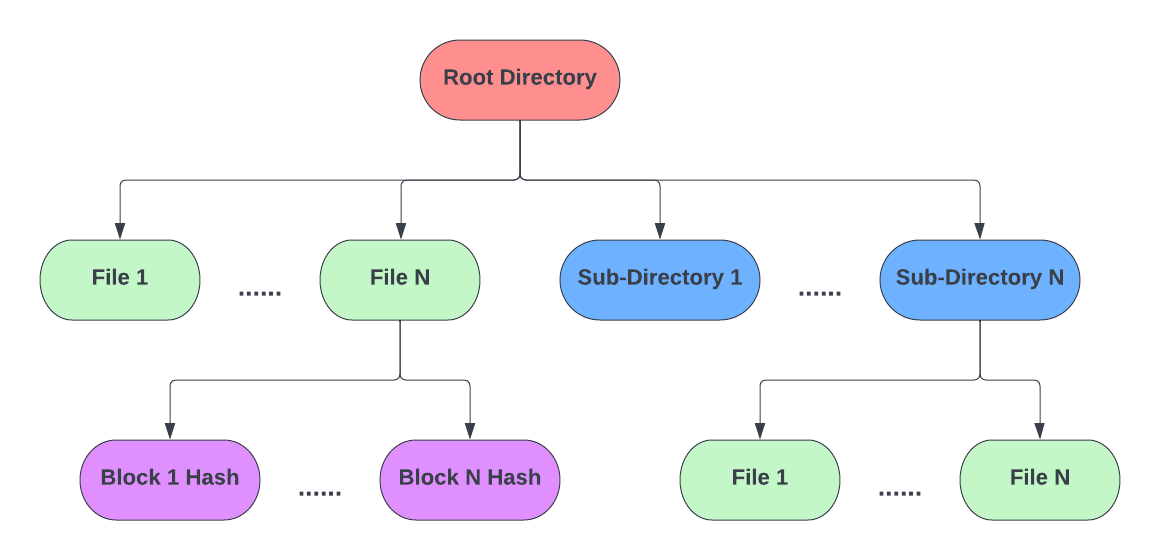
\includegraphics[width=.85\textwidth]{assets/images/diagrams/block-body.png}
  \caption{The structure of a hash tree}
  \label{fig:hash-storage}
\end{figure}

\subsubsection*{Uploading Content}
\label{subsubsec:upload-content}

For a developer to upload their game \reqref{F-M1}, they must provide the following:

\begin{itemize}
  \item the metadata outlined in Section~\ref{subsubsec:eth-data},
  \item a hash tree created from the root directory of the game, and
  \item an assets folder containing a piece of cover art \textit{(cover.png)} and a description file \textit{(description.md)}.
\end{itemize}

\vspace{2mm}\noindent
The developer should be able to enter the required fields into an upload page of the GUI and have the data generated and uploaded for them \reqref{F-S2}.

\subsubsection*{Downloading Content}

\newcommand{\seeder}{$P_{seeder}$~}
\newcommand{\downloader}{$P_{downloader}$~}

Like mentioned in Section~\ref{subsec:design-data}, it is impractical to store the game's data on the blockchain or IPFS. Instead we will consider ideas from decentralised file-sharing networks, like discussed in Sections~\ref{sec:lit-p2p} \&~\ref{sec:bittorrent}.
\x
Games are content addressable using their root hash field, which will allow users to request data from that game from other users. When a peer seeking data \downloader forms a connection with another peer \seeder they will:

\begin{enumerate}
  \item Perform a handshake to determine each other's Ethereum address and public key.
  \item \seeder will verify that \downloader owns the game by checking the \textit{purchased} mapping on the smart contract \reqref{F-M6} \reqref{F-S1}.
  \item \downloader will send requests for individual blocks to \seeder \reqref{F-M9}.
  \item Upon receiving a block, \downloader will verify the contents using the block's hash \reqref{F-M10} before writing it to disk in the appropriate location.
  \item Repeat Steps 3--4 until the entire game has been downloaded \reqref{F-M11}.
  \item \seeder may request a signed receipt that details the blocks they uploaded \reqref{F-S3} to \downloader.
\end{enumerate}

\vspace{2mm}\noindent
Users will be able to connect to many peers at once \reqref{F-M7} and will send download requests to the subset of their peers who also own the game. Requests will be sent in a round-robin fashion to evenly distribute the requests and prevent overloading a single peer \reqref{NF-S1}. Requests that cannot be completed will be retried when connecting to a new peer or when a peer has a change in library.

\subsubsection*{Updating Content}\label{subsubsec:updating}

To satisfy \reqref{F-M2}, developers will perform the same steps outlined in Section~\ref{subsubsec:upload-content} but must also provide the root hash of the most previous version of the game. Any users who have purchased the previous version will be added to the list of users who have purchased the new version \reqref{F-M3}. Additionally, this will include the restriction that only the original uploader can upload an update for their game \reqref{NF-M5}.
\x
Each version is considered its own game and will require users to download the updated version separately. Whilst this isn't reflective of how updates are typically managed, this will be acceptable for the scope of this project.

\subsubsection*{Downloadable Content}

Downloadable Content (DLC) \reqref{F-C1} represent optional additions for games that users will buy separately. DLCs will act similarly to how updates are treated. Each DLC will need:

\begin{enumerate}
  \item \textbf{Dependency} The root hash of the oldest version of the game this DLC supports.
  \item \textbf{Previous Version} (Optional) The root hash of the previous version of the DLC.
\end{enumerate}

\vspace{2mm}\noindent
Users must own the original game to buy any of its DLC. 

\subsubsection*{Proving Contribution}

As a user downloads blocks of data, they will keep track of which users have sent them which blocks. A peer may then request their contributions in the form of a signed message that can be sent to the developer \reqref{F-S3} in return for some kind of reward. The contents of the reward isn't specified for this project but could include in-game items, digital assets or Ether. This solution assumes that developers have knowledge of which Ethereum address maps to which of their game's users.

\section{Architecture}

This application uses the Model-View-Controller MVC pattern to structure the application to create a separation of concern between the main layers of the application. Figure~\ref{fig:impl-layers} shows a high level overview of the architecture and below I discuss the purpose for each.

\begin{figure}[ht]
  \centering
  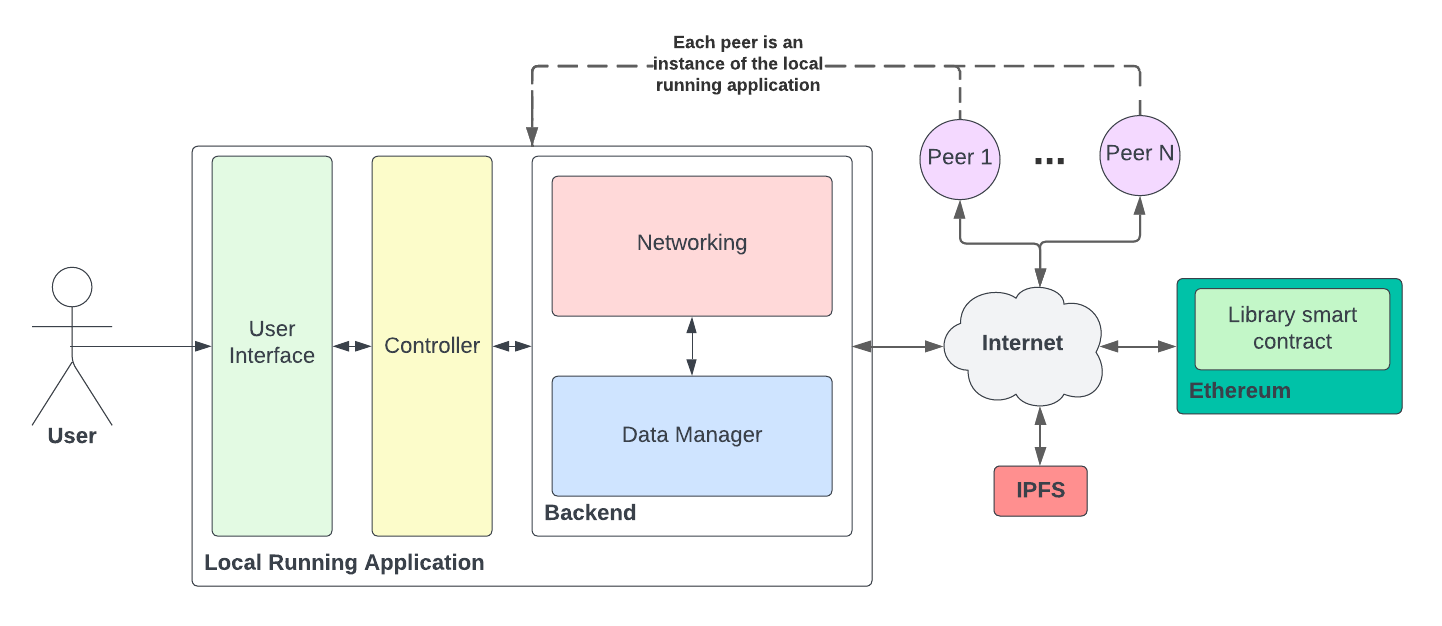
\includegraphics[width=.8\textwidth]{assets/images/diagrams/layers.png}
  \caption{The layers of the application}
  \label{fig:impl-layers}
\end{figure}

% layer entries


\subsection{Persistence}

The Persistence layer shows how the data for the application is divided across several mediums; namely the \textbf{Ethereum Smart Contract}, \textbf{IPFS}, and a \textbf{P2P Network}. Each component stores a different, which is outlined in Section~\ref{subsec:design-data}.
\x
There are several things to note about using Ethereum as platform for selling games:

\begin{itemize}
  \item Ethereum is a less stable currency than most traditional currencies like GBP or USD so games may fluctuate largely in price.
  \item All write functions on the smart contract will incur a gas fee so uploading or updating data will not be free.
  \item Users will have to source Ether from elsewhere before being able to purchase games, which may be intimidating to users not already familiar with the ecosystem.
\end{itemize}

% \subsubsection{Ethereum}\label{subsubsec:impl-eth}

% An Ethereum Smart Contract, written in Solidity \url{https://docs.soliditylang.org/en/v0.8.19/}, will be used to store the set of data about games that is required for the identification of each game. The Smart Contract will also be used to perform the following:
% \x
% The Geth go-ethereum package \url{https://geth.ethereum.org/} will allow us to interact with the ethereum blockchain and Abigen \url{https://docs.avax.network/specs/abigen} will allow us to compile any smart contracts to Go code. This will allow us to interact with our smart contract on ethereum using a set of Go functions. For development, Ganache \url{https://github.com/trufflesuite/ganache} was used to create a local Ethereum instance and Geth was used to connect to an Ethereum test net.


% \subsubsection{IPFS}

% This project will use the IPFS implementation Kubo \url{https://github.com/ipfs/kubo}, due to it being the most widely used implementation of IPFS. We will use the go-ipfs-api library \url{https://github.com/ipfs/go-ipfs-api} to interact with Kubo and upload/download the data specified above.


\subsection*{Backend}\label{subsec:backend}

The Backend can be broken down into two major components:

\begin{itemize}
  \item \textbf{Networking} The creation and maintenance of network connections with other peers over the internet with the purpose of sharing data.
  \item \textbf{Data Manager} the management of local data and the processing of data received and to be uploaded by the Networking component.
\end{itemize}

\input{sections/5-design/components/backend/networking.tex}
\input{sections/5-design/components/backend/manager.tex}
\input{sections/5-design/components/backend/optimisations.tex}

\subsection*{Frontend \& Controller}

\subsubsection{Frontend}\label{subsubsec:frontend}

This application will have a GUI \reqref{F-S2} \reqref{NF-S2} where users can interact with the platform. Having a GUI is essential to making the platform as easy to use as possible so that it is accessible to new users. At minimum it will need to include the following pages:

\begin{itemize}
  \item \textbf{Library} The user's collection of owned games, where they can view details for each game as well as manage their download status.
  \item \textbf{Store} Where user's can find and purchase new games that have been uploaded by other users.
  \item \textbf{Upload} Where users can fill in details about their new or updated game and have it be uploaded to the network.
  \item \textbf{Downloads} Where user's can track all of their ongoing downloads and see their progress.
  \item \textbf{Peers} Where users can manage their list of connected peers. Here a user can form new connections, break existing ones and request specific data from their peers.
  \item \textbf{Help} A help page to describe the application and all of its functionality \reqref{NF-C1}
\end{itemize}

\newparagraph
To satisfy \reqref{NF-M3}, a developer must always be displayed with both their chosen name and their Ethereum address. A developer should publically provide their Ethereum address to ensure their users can identify it.

\subsubsection{Controller}

The Controller will be represented as a set of interface functions that allow the backend and frontend code to communicate. This can be done to trigger actions such as starting a game download or to fetch data like the list of a user's owned games.


\newpage

\section{Downloading a Game}

Figure~\ref{fig:p2p-interactions} shows the standard sequence of events used for a user to download a game from this application. The developer will upload a game that is purchased by a user; this user will then proceed to download the game off of the developer using the commands described in Section~\ref{subsubsec:commands}.
\x
Some important notes about this interaction are:

\begin{itemize}
  \item Identity verification happens immediately after forming a connection.
  \item Deferred requests are attempted when connecting to a new peer and after a timeout.
  \item Game ownership is checked upon the first BLOCK request.
\end{itemize}

\begin{figure}[!ht]
  \centering
  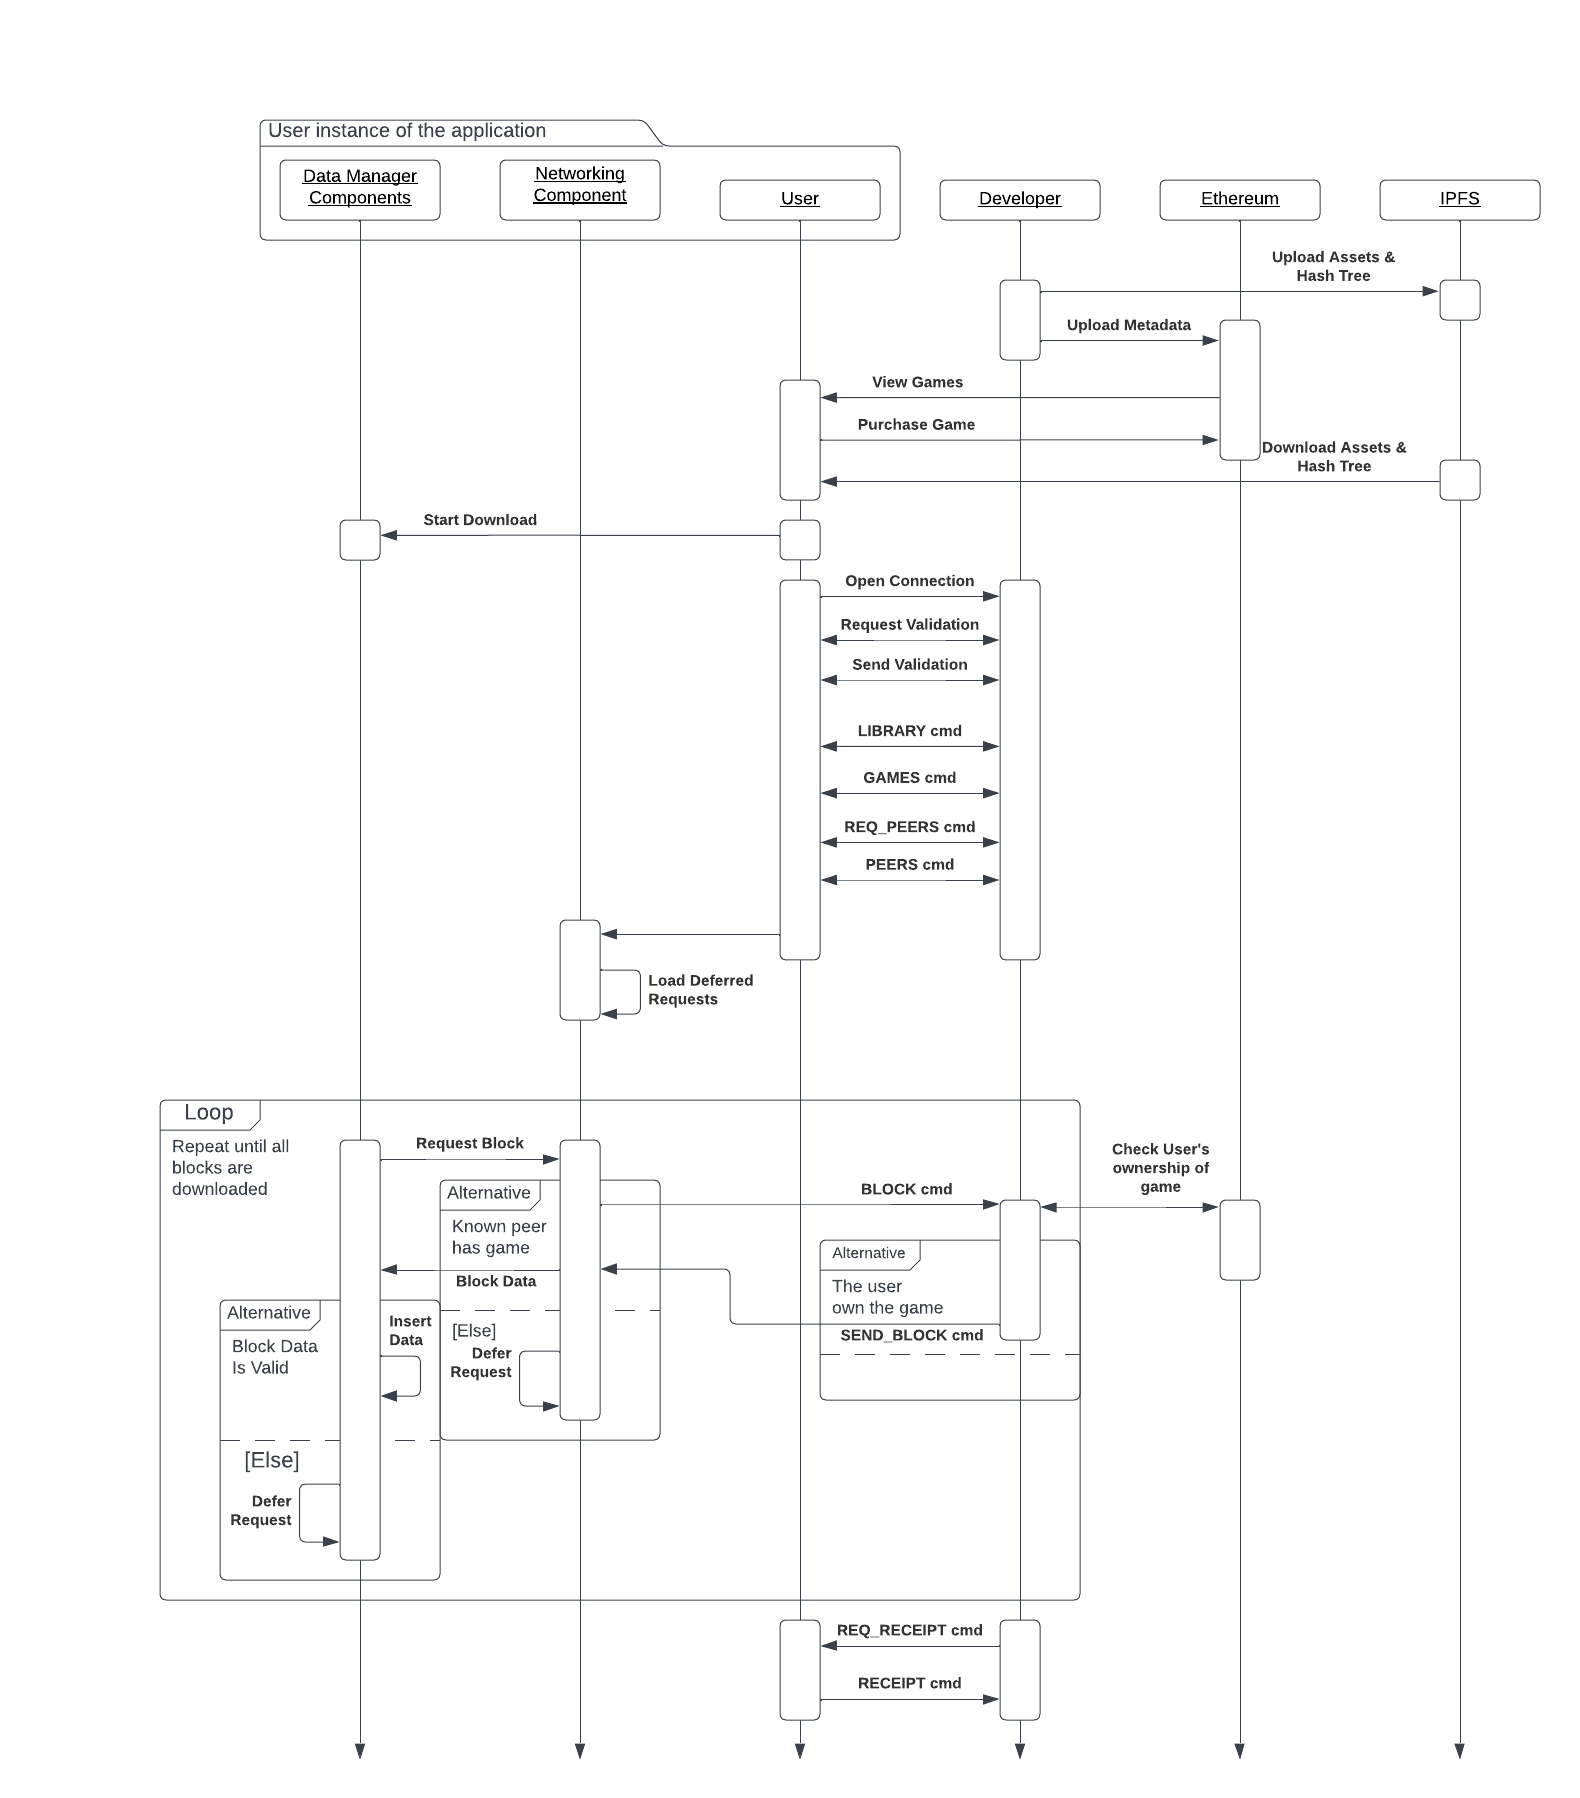
\includegraphics[width=\textwidth]{assets/images/diagrams/p2p-sequence.png}
  \caption{A sequence diagram showing the main interactions needed to download a game}
  \label{fig:p2p-interactions}
\end{figure}



\section{Benefits}\label{des:benefits}

This application presents the following benefits when compared with centralised game marketplaces:

\begin{itemize}
  \item \textbf{Privacy} A user's personal information and usage isn't collected. Traditional platforms require users to enter personal information and will actively collect data about a user's actions through the platform.
  \item \textbf{Ownership} A user's ownership of a game isn't tied to a single platform and use of Ethereum means that a user's ownership is upheld by all computers in the network.
  \item \textbf{Censorship} Similar to the previous point, no one party has control over the platform so it is much harder for third parties, such as governments, to restrict the content uploaded to it.
  \item \textbf{Profits} Developers and gamers communicate directly and this means developer's won't have to pay a hefty fee for a middle-man. This will result in potentially larger profits for the developers.  
\end{itemize}

\section{Limitations}\label{sec:design-lim}

This application presents the following limitations when compared with a centralised game marketplace:

\begin{itemize}
  \item \textbf{No Social Features} Social features, such as friends or achievements, were not included within the scope of this project.
  \item \textbf{Availability} Section~\ref{subsec:availability} highlights the issue of availability within P2P file-sharing systems and it is likely this platform will face similar issues.
  The use of a contribution system was implemented to help identify those users who have been contributing but there is no automatic rewards system\footnote{An example would be how the micro-payment system works in Swarm~\cite{hartman_swarm_1999}}.
  \item \textbf{Inefficient Updates} As updates are treated as individual games, they will require users to download the entire game again. This is highly inefficient and results in lots of duplicate data being downloaded.
  \item \textbf{Illegal Content} Currently there is no policy, automated or otherwise, to stop the distribution of illegal content. This is an incredibly complex problem to tackle and any obvious solution would risk violating the anti-censorship goal of this project. 
\end{itemize}